%%%%%%%%%%%%%%%%%%%%%%%%%%%%%%%%%%%%%%%%%%%%%%%%%%%%%%%%%%%%%%%%%%%%%%%%%%%%%%%%
%2345678901234567890123456789012345678901234567890123456789012345678901234567890
%        1         2         3         4         5         6         7         8

\documentclass[letterpaper, 10 pt, conference]{ieeeconf}  % Comment this line out if you need a4paper

%\documentclass[a4paper, 10pt, conference]{ieeeconf}      % Use this line for a4 paper

\IEEEoverridecommandlockouts                              % This command is only needed if 
\usepackage{graphicx}
\usepackage{caption}
\usepackage{subcaption} % you want to use the \thanks command
\usepackage{multirow}
\usepackage{multicol}
\usepackage{graphicx}
\usepackage{nomencl}
\usepackage{amsmath, xparse}
\usepackage{amsmath,amssymb}
\usepackage{caption}
\usepackage{subcaption}
\usepackage{tabularx}
\usepackage{mathtools, nccmath}
\usepackage{lipsum}
\usepackage{romannum}
%\usepackage[demo]{graphicx}
\usepackage{comment}
\usepackage{hyperref}
%\usepackage[margin=1.5cm]{geometry}
\usepackage{graphicx,subcaption,lipsum}
\usepackage{array}
\usepackage{booktabs}
\usepackage[table]{xcolor}
\usepackage{xcolor}


                                                        % you want to use the \thanks command
\overrideIEEEmargins                                      % Needed to meet printer requirements.

%In case you encounter the following error:
%Error 1010 The PDF file may be corrupt (unable to open PDF file) OR
%Error 1000 An error occurred while parsing a contents stream. Unable to analyze the PDF file.
%This is a known problem with pdfLaTeX conversion filter. The file cannot be opened with acrobat reader
%Please use one of the alternatives below to circumvent this error by uncommenting one or the other
%\pdfobjcompresslevel=0
%\pdfminorversion=4

% See the \addtolength command later in the file to balance the column lengths
% on the last page of the document

% The following packages can be found on http:\\www.ctan.org
%\usepackage{graphics} % for pdf, bitmapped graphics files
%\usepackage{epsfig} % for postscript graphics files
%\usepackage{mathptmx} % assumes new font selection scheme installed
%\usepackage{times} % assumes new font selection scheme installed
%\usepackage{amsmath} % assumes amsmath package installed
%\usepackage{amssymb}  % assumes amsmath package installed

\title{\LARGE \bf Automated Vision-based Bolt Sorting by Manipulator for Industrial Applications}


\author{Surya Prakash S.K$^{1}$ Amit Shukla$^{2} $  Naisarg Pandya$^{3}$ Shirish Shekhar Jha$^{4}$% <-this % stops a space
\thanks{*This work was not supported by any organization}% <-this % stops a space
\thanks{$^{1}$ Surya Prakash S.K Author is, Research Scholar, School of Mechanical and Materials Engineering, IIT Mandi, Himachal Pradesh, India.}%
\thanks{$^{2}$Amit Shukla, Chairperson Centre for Artificial Intelligence and Robotics, IIT Mandi, Himachal Pradesh, India.}
\thanks{$^{3}$ Naisarg Pandya, Research Scholar, School of Mechanical and Materials Engineering, IIT Mandi, Himachal Pradesh, India.}
\thanks{$^{4}$ Shirish Shekha Jha, Research Intern, Centre for Artificial Intelligence and Robotics, IIT Mandi, Himachal Pradesh, India.}
}

\begin{document}

\maketitle
\thispagestyle{empty}
\pagestyle{empty}


%%%%%%%%%%%%%%%%%%%%%%%%%%%%%%%%%%%%%%%%%%%%%%%%%%%%%%%%%%%%%%%%%%%%%%%%%%%%%%%%
\begin{abstract}
In industrial automation, nuts and bolts are key components that facilitate assembly processes. Estimating their sizes and sorting them accordingly would be a significant advancement for automation in industrial settings. This paper introduces a distinct approach by amalgamating deep learning based segmentation with classical vision for automated bolt sorting in unstructured industrial environment. We evaluated advanced deep learning algorithms PPLiteSeg(STDC I\&II), OCRNet, and DeepLabV3+ on our custom bolt dataset. DeepLabV3+ achieved the best performance over the other models in accurate bolt segmentation, with a remarkable mean Intersection over Union (mIoU) of 0.95. Custom bolt dataset is prepared considering various environmental conditions and included both new and aged bolts. We present a comparative analysis of the segmentation results for each learning model mentioned. To estimate bolt size, we integrated the segmented binary image with depth information from Intel RealSense D415 camera. Through a series of experiments, we successfully localized bolts (both position and orientation) relative to robot’s base and sorted them according to their size by using Kinova Gen3 Lite robotic arm. The proposed approach has the potential to significantly advance the automation for assembly lines and warehouse management within industries, particularly when dealing with small objects.
\end{abstract}


%%%%%%%%%%%%%%%%%%%%%%%%%%%%%%%%%%%%%%%%%%%%%%%%%%%%%%%%%%%%%%%%%%%%%%%%%%%%%%%%
\section{INTRODUCTION}
In automation and warehouse management industries, the involvement of robots will reduce human effort and improve the efficiency of tasks by eradicating human fatigue and mistakes. In the above-mentioned industries, robots are generally used for picking up objects and placing them in their designated place. The degree of automation can be defined as the extent to which this process is carried out autonomously. Generally, robots perform manipulation tasks in structured environments where objects' positions are predefined. For unstructured environments, a vision-based approach for object localization in manipulation tasks has been introduced. Generally, localization of objects using classical vision techniques such as markers, edge detection, corner detection, and contour detection may not be reliable for all situations. For example, under varying light conditions, shapes, and colors, these classical methods may underperform in localization, consequently resulting in faulty localization and size estimation. \cite{DeepLearningvsClassicalVision}.

On the other side, we can observe how humans generally use their perception to complete tasks. In brief, when we first identify an object, we rely on our previous knowledge to recognize its shape and texture, allowing us to conclude which category it belongs to. After that, either by visually assessing the object or by physically handling it, we can estimate its size. However, this process is skill-based and prone to mistakes. If there were a way to integrate human perception and classical vision techniques to estimate size in random environments with fewer mistakes, it would represent a significant advancement in automation.

Recent advancements in deep learning, particularly Convolutional Neural Networks (CNNs), offer promising solutions for overcoming the limitations of classical vision methods. CNNs can learn to extract relevant features from images, even for small objects with limited details. This capability, combined with sensor fusion techniques, can provide a more robust understanding of object size and shape. This integration of CNNs with classical vision methods not only facilitates feature extraction for small and limited-featured objects but also helps to estimate object size accurately, thereby streamlining subsequent actions based on the detected size. The challenges in this task include: (1) overcoming lighting conditions and cluttered environments in the factory setup, (2) extracting features from small and less-featured objects (bolts), (3) dealing with color variations (old and new bolts), (4) precise size estimation of small objects (bolts), and (5) integrating the perception module (Deep Learning + Classical Vision) with the robot.

This paper presents a systematic approach for automated bolt sorting using deep learning and depth information. Following the introduction in Section I, Section II provides a comprehensive review of related work in the field of automated bolt sorting and object classification using deep learning techniques. Section III details the proposed methodology, outlining the specific steps involved, including data acquisition, the custom dataset size used for the segmentation model, semantic segmentation with DeepLabV3+, size estimation using depth information, and robot arm control. Section IV describes the experimental setup, including our system's specifications, and presents the results achieved by the proposed system. Finally, Section V concludes the paper by summarizing the key findings, highlighting the potential impact of this work on industrial automation, and discussing our future extensions of the present work. 
\newpage
\section{RELATED WORK}
Automated bolt size estimation and sorting in unstructured environment will require the integration of 4 components.
\begin{itemize}
    \item Object Segmentation (CNNs)
    \item Size Estimation (Classical Vision)
    \item Localization in Robot's configuration
    \item Robot Reaching to Localized Bolts
\end{itemize}

Object/image segmentation is a fundamental technique in computer vision, aiming to partition an image into distinct regions based on the class or category to which each pixel belongs. In \cite{INSVSSEM}, the authors explain that there are two ways to achieve segmentation: instance segmentation and semantic segmentation. Instance segmentation, in our case, would classify all bolts within the cluttered image and assign a unique color and label to each bolt. On the other hand, semantic segmentation would classify the bolts and assign a unique label and color to all bolts in the image. However, our objective is to sort the bolts according to their size, and we may not require a unique label for each bolt in the image. Therefore, using semantic segmentation in our case will simplify the segmentation process and reduce computational complexity. \cite{StateofArtSemanticSegmentation} Gives a comprehensive review on classical 2D image segmentation models. Models like FCN, DeepCovnNet, U-Net, SegNet, DeepLabV1 to DeepLabV3+ \cite{FCN, DeepCOnvNet, U-Net, segnet, DeepLabV1, DeepLabV2, DeepLabV3, DeepLabV3+} are CNN encoder-decoder architecture models are best performed for classical image segmentation. \cite{PPLiteSeg} PPLiteSeg (STDC I \& II) are lightweight CNN architectures designed for real-time applications in resource-constrained environments. Furthermore, \cite{OCRNET} OCRNet, a model that leverages an object-contextual representation approach, demonstrating the potential benefits of exploring techniques beyond classical CNN-based architectures.
 
Size estimation from 2D segmented images, leveraging classical vision techniques, is another key component. In \cite{DeepLearningvsClassicalVision}, the authors compared traditional classical vision methods with deep learning methods, highlighting the advantages of integrating both approaches. They explained how the combination can enhance computer vision perception, leading to more robust and accurate results. For instance, deep learning-based object detection by YOLO bounding box dimensions and aspect ratio can be used to estimate object size with some success, as demonstrated in \cite{RGBD} using RGBD cameras for human height estimation. However, in our case, we leverage a deep learning-based object segmentation method. This approach, using classical vision on segmented objects, provides more accurate object boundaries compared to direct bounding boxes by object detection. Hence, our approach leads to accurate size estimation and eliminates the influence of background clutter on size measurements.

Localization of object in image frame and transforming it to robot's configuration is another key component. \cite{projective} explains the camera projective transformations, which is a classical method to transform object co-ordinates in pixels to the camera coordinate frame in metric units.Another important component is enabling the robot arm to reach the object's location for the required sorting task. In \cite{stonesize}, size estimation of unknown shapes (stones) uses classical vision techniques such as color thresholding to separate stones from the background. After masking, the image is aligned with the corresponding RGBD point cloud data to estimate the stone size. However, classical vision-based segmentation suffers from background changes, lighting variance, and faulty detection in the case of stone-like objects. In \cite{F-RCNN} authors used Mask R-CNN to achieve both object detection and instance segmentation in one step, obtaining precise bounding boxes and segmentation masks for accurate grasping. \cite{FRCNN} Introduces a Faster R-CNN-based approach achieving 0.9644 mAP for automated hardness detection in aircraft bolts. \cite{CNN} Investigates efficient joint and bolt identification using a CNN, highlighting superior performance over traditional methods. \cite{Hough} Presents a circle detection method based on Hough transform for bolt diameter computation in manufacturing scenarios. \cite{NUTBOLT} Deploys an ANN-based Back propagation Neural Network to distinguish nuts and bolts on a moving platform. \cite{DomainRandomization} Proposes a machine learning solution utilizing synthetic data for precise bolt detection in aircraft fuselage layer joining under varying real-world conditions. In \cite{editor} The paper introduces a hybrid system merging CNN-based object detection with VGG16's RPN and classical pose estimation using SIFT and RANSAC-ICP algorithms. Achieving accurate localization and pose estimation, it suffers from longer inference times (0.9s for detection, 1s for pose) and relies on rich-textured objects. In contrast, our method, using DeepLabv3+ for segmentation, achieves faster inference (130ms) with broader applicability.

Contrary to previous works that focus on objects rich in features and geometrically distinct from one another, our approach aims to develop a robust method for automating the sorting of objects with fewer features, such as bolts. We have carefully created data for model training in random environments, ensuring versatility and robustness. Our method achieves a 0.95 mIOU for segmentation with an inference time of 130 ms. By incorporating depth data, we can accurately estimate bolt sizes, a critical aspect that enhances precision in sorting.
\section{Methodology}
\begin{figure}[h!]
\centering
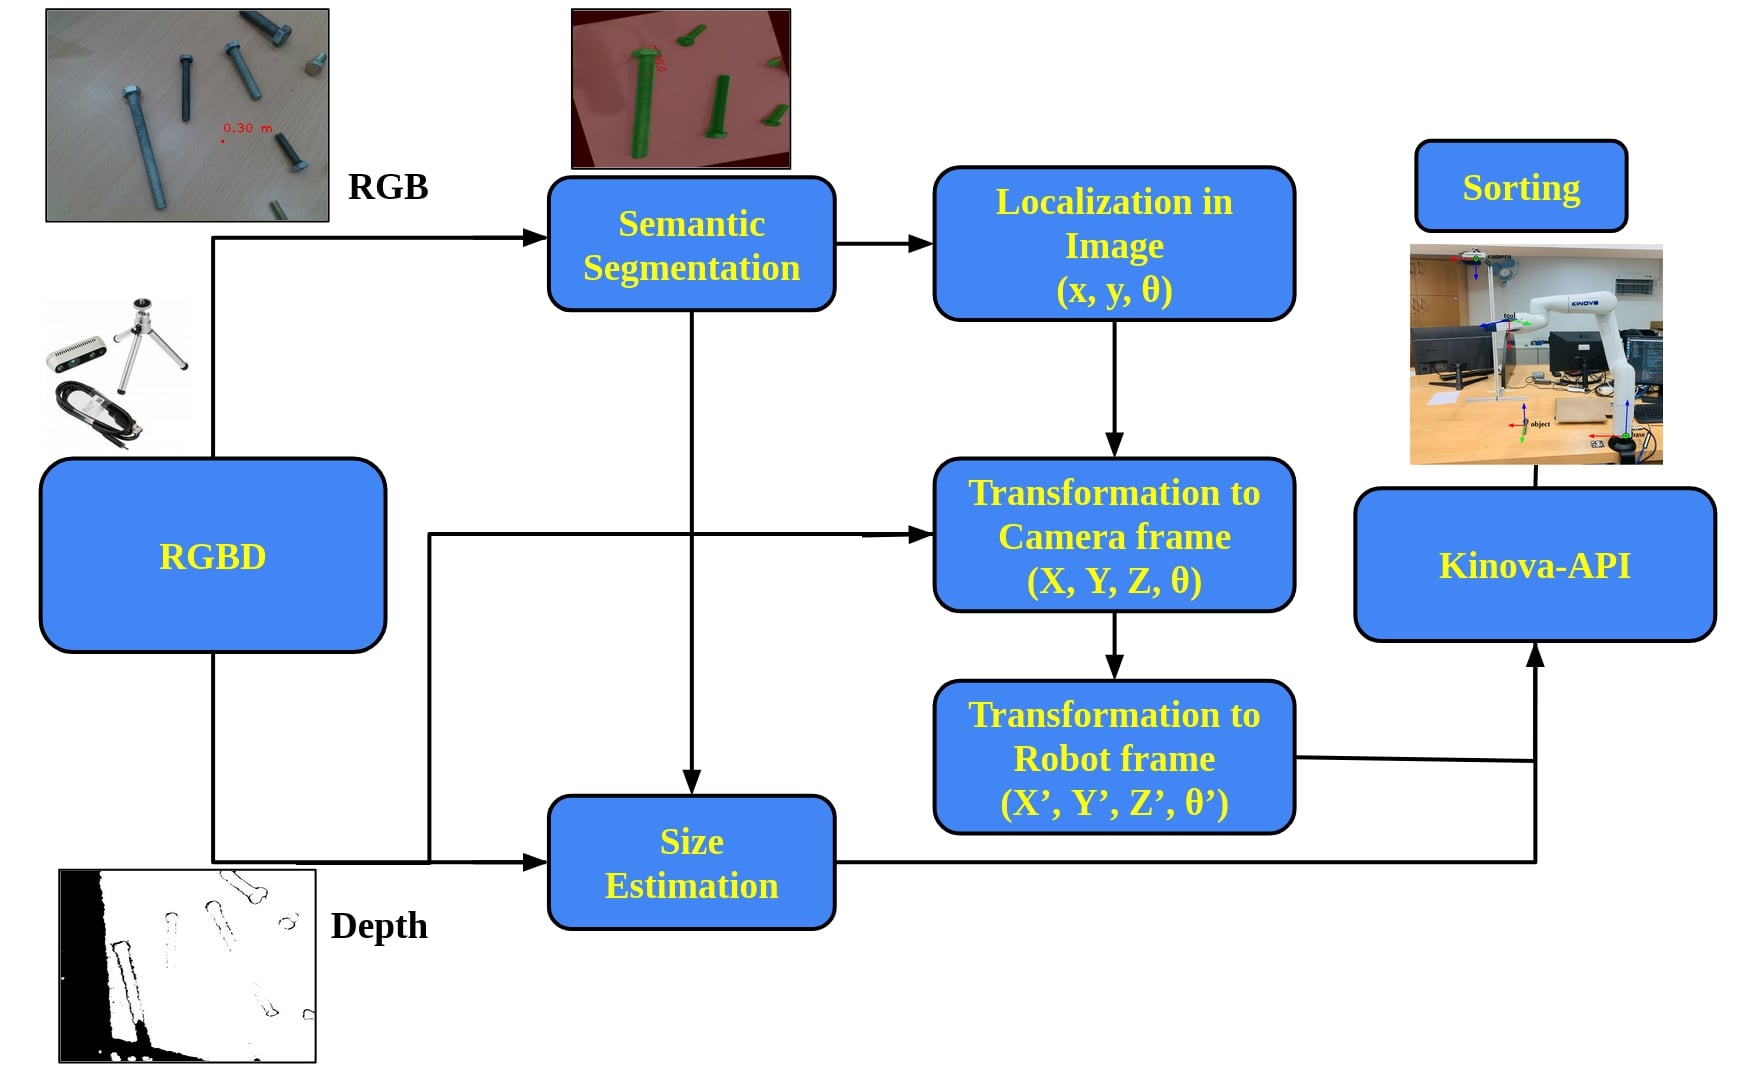
\includegraphics[width=\columnwidth]{overall_methodology.jpg}
%\epsfxsize=3.25in\epsfbox{figure1.epsi}
\caption{Overall methodology.}
\label{methodology}
\end{figure}
Our methodology, as shown in Fig. \ref{methodology}, begins by capturing RGB and depth frames using a depth camera fixed at a predefined global position. The RGB frame is directed to a semantic segmentation model, and upon segmentation of the RGB image, the corresponding depth frame is aligned. Using classical vision techniques, we accurately estimate the size of the bolts. In the context of robot arm control for grasping, precise localization of each bolt's position and orientation relative to the robot's base frame is crucial. To achieve this, we first localize each bolt in the segmented image, obtaining its position in pixel coordinates relative to the image frame. To enable interaction with the real world, we leverage the depth information from the RGB-D camera, which provides depth measurements in metric units (meters). This depth information, along with the intrinsic camera parameters and the initial pixel-based localization of the bolt in the segmented image, allows us to convert the pixel coordinates into metric coordinates within the camera frame. Hence, with the robot and global camera positioned in predefined locations, we can transform coordinates in the camera frame to the robot base frame. Leveraging the Kinova API, we transmit the final bolt localization data (position and orientation) to the robot arm as control inputs (X', Y', Z', $\theta$), enabling the arm to precisely grasp and sort the bolts based on their estimated size.
\subsection{Data Collection \& Annotation}
Our first step in achieving the task is to collect data to train our models for image segmentation. In the process of data collection, we have considered real-time environmental conditions such as different backgrounds (green, blue, black, cemented tiles, wooden table colors) and varying light conditions (different sunlight, varying lights in the laboratory) along with new and aged bolts. Our study is confined to Mild Steel (M.S) bolts, this decision is based on the prevalence of M.S bolts in industrial environments. The collected images are labeled as bolts using the Roboflow platform, as shown in Fig. \ref{fig:combined_figures}. Our image dataset (480 × 640) consists of 2000 images, including augmentations. The dataset is further split into training, test, and validation sets in percentages of 80, 10, and 10, respectively.
\begin{figure}[h]
    \begin{subfigure}{0.2\textwidth}
        \centering
        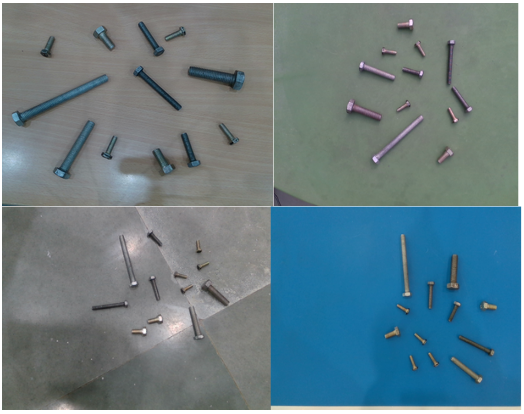
\includegraphics[width=1\linewidth]{paper_1.png}
        \caption{}
        \label{fig:figure_a}
    \end{subfigure}
    \hfill
    \begin{subfigure}{0.2\textwidth}
        \centering
        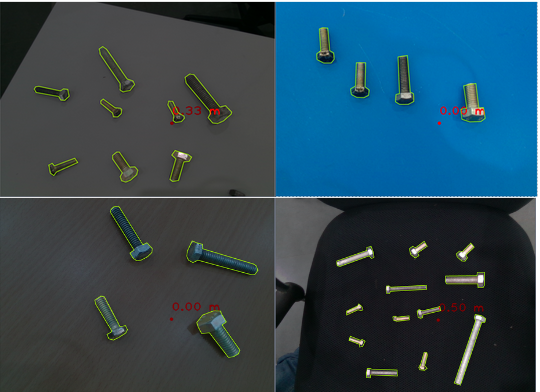
\includegraphics[width=1.05\linewidth]{paper_2.png} 
        \caption{}
        \label{fig:figure_b}
    \end{subfigure}
    \caption{(a) Data collection (b) Annotations of collected images.}
    \label{fig:combined_figures}
\end{figure}

\subsection{Bolt Segmentation}
Semantic segmentation plays a crucial role in our methodology by separating bolts from the background in images. We created a bolt dataset considering real-world environmental factors and fed it into a semantic segmentation model. We evaluated various standard CNN architectures on our custom dataset. A detailed comparison of their performance parameters is presented in TABLE \ref{comparision_deep}.
PP-LiteSeg, with its encoder-decoder architecture featuring FLD, UAFM, and SPPM modules, excels in general image segmentation tasks. However, in our specific case of bolt segmentation, due to their small size, PP-LiteSeg struggles and generates inaccurate segmentation masks. OCRNet, utilizing the HRNet48w architecture, excels at capturing fine details with its multi-resolution fusion and OCR module. While this allows for effective segmentation of small objects like bolts, variations in lighting and bolt textures can still lead to inconsistent segmentation results. DeepLabV3P, featuring a ResNet101 backbone, utilizes dilated convolutions and atrous spatial pyramid pooling (ASPP) for efficient context capture at various scales. Therefore, DeepLabV3P is particularly effective for semantic bolt segmentation due to its capacity to reliably capture fine details and spatial context, which is crucial for identifying bolts from their surroundings. ASPP's multi-scale context aggregation ensures that bolts of diverse sizes and orientations can be reliably segmented, making the model resistant to common bolt combinations found in industrial settings. Furthermore, the depth of ResNet101 allows the model to acquire detailed features and representations, further improving its segmentation performance on complex bolt images.
\begin{figure}[h!]
\centering
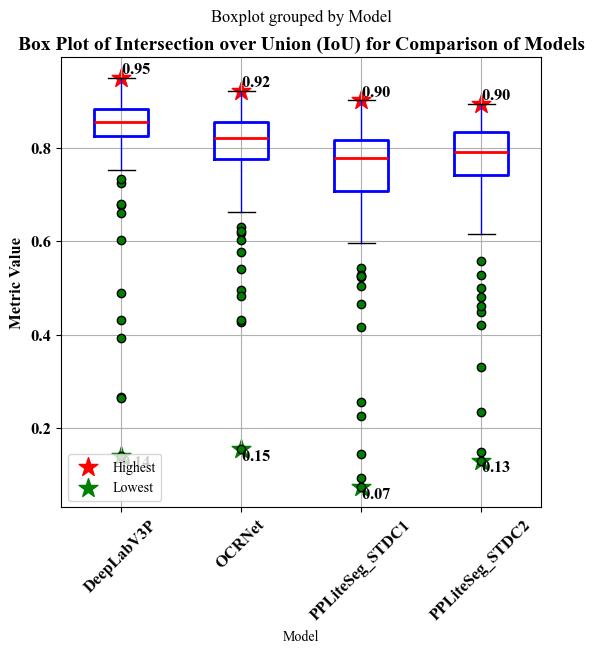
\includegraphics[width=0.75\columnwidth]{iou_comparison.png}
%\epsfxsize=3.25in\epsfbox{figure1.epsi}
\caption{Comparison between models with IoU metric.}
\label{comparison_1}
\end{figure}
The evaluation of Intersection over Union (IoU) scores from Fig.\ref{comparison_1} in the semantic segmentation of bolt images offers valuable insights into the performance of the segmentation models. Lower IoU scores indicate poorer alignment between predicted and ground truth segmentation masks. This misalignment can be attributed to various factors, such as backgrounds with colors similar to bolts, extended shadows obscuring bolt boundaries, and augmented images containing unrealistic variations not present in the training data.

\begin{figure}[h!]
\centering
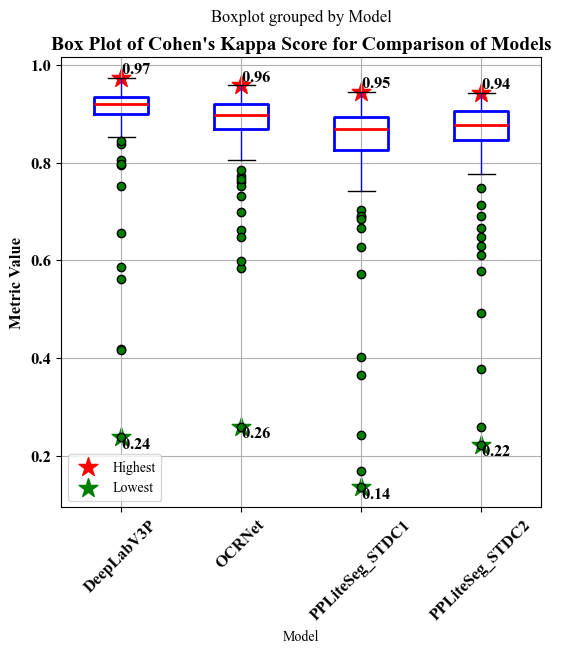
\includegraphics[width= 0.75\columnwidth]{kappa_comparison.png}
%\epsfxsize=3.25in\epsfbox{figure1.epsi}
\caption{Comparison between models with Kappa-Coherence score metric.}
\label{comparison_2}
\end{figure}
Lower Kappa scores from Fig.\ref{comparison_2}, denoting weaker agreement between predicted and ground truth segmentation, have manifested due to several underlying factors. One notable factor contributing to this trend is the complexity of bolt structures and their surrounding environments, which may introduce ambiguity and variability in segmentation interpretations. Additionally, the presence of subtle visual cues, such as intricate surface textures or irregular lighting conditions, might have further exacerbated segmentation difficulties, leading to decreased Kappa scores.
\begin{table*}[htbp]
\caption{Comparison of Models for Bolt Segmentation of Custom Bolt Data}
\begin{center}
\renewcommand{\arraystretch}{1.2} % Adjust row height
\rowcolors{2}{gray!25}{white} % Alternate row colors
\begin{tabular}{|>{\centering\arraybackslash}m{2.5cm}|>{\centering\arraybackslash}m{2.5cm}|>{\centering\arraybackslash}m{2.5cm}|>{\centering\arraybackslash}m{2.5cm}|>{\centering\arraybackslash}m{2.5cm}|}
\hline
\textbf{Model Name} & \textbf{PPLiteSeg I} & \textbf{PPLiteSeg II} & \textbf{DeepLabV3P} & \textbf{OCRNet} \\
\hline
\textbf{Backbone} & STDC I & STDC II & ResNet101\_vd & HRWNet\_48w \\
\hline
\textbf{mIoU} & 0.8921 & 0.8964 & 0.92 & 0.9135 \\
\hline
\textbf{Model Size (MB)} & 31.8 & 47.2 & 174 & 268 \\
\hline
\textbf{Loss Function} & OHEM Cross Entropy & OHEM Cross Entropy & OHEM Cross Entropy & OHEM Cross Entropy \\
\hline
\textbf{Inference Time (ms)} & 228 & 330 & 131 & 275 \\
\hline
\textbf{Dice Coefficient} & 0.9399 & 0.9427 & 0.9568 & 0.953 \\
\hline
\textbf{Kappa Score} & 0.8797 & 0.8855 & 0.9136 & 0.906 \\
\hline
\end{tabular}
\label{comparision_deep}
\end{center}
\end{table*}



\subsection{Bolt Localization \& Size Estimation  }
After segmentation of bolts from the RGB frame of size (480, 640) and the corresponding depth frame of (480, 640) is aligned, with assistance of classical vision, ($c_{x}, c_{y}$) denotes the centroid of the 2D segmented object in the image. Correspondingly, ($x_{p}, y_{p}$) represents the center of the image \textbf{(240, 320)} in our case. The bounding box width on each segmented bolt, as shown in Fig. \ref{size_estimation}, will give the dimension of the bolt head. The orientation of each bolt is determined from the inclination of the longest side of the bounding box with a horizontal line parallel to the \textbf{u} axis. In Eq. \ref{dia_pixel-equ}, $D_{p}$ represents the bolt head diameter, and $d_{p}$ represents the shank diameter in pixels and $d_{m}$ is shank diameter in metric units. Intrinsic parameters obtained from calibration, along with depth from the camera, are used to transform localized pixel coordinates to metric coordinates, as shown in Eq. \ref{coordinate_equations} and the estimated bolt diameter for several samples is shown in TABLE. \ref{Table2}.

\begin{equation}
    \centering
    d_{p} = \frac{D_{P}}{1.8}, \hspace{1cm} \textnormal{size} = d_{m} = \frac{d_{p}}{f\cdot\rho}\cdot Z.
\label{dia_pixel-equ}
\end{equation}
where 'f' is the focal length in m, \newline
'$\rho$' is number of pixels per unit length in pixel/m.
\begin{figure}[h!]
\centering
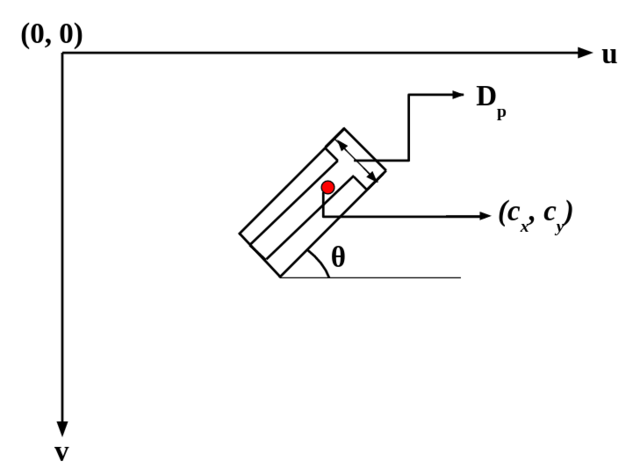
\includegraphics[width=0.5\columnwidth]{size_estimation.png}
%\epsfxsize=3.25in\epsfbox{figure1.epsi}
\caption{Feature extraction from segmented bolt image.}
\label{size_estimation}
\end{figure}

\begin{equation}
    \centering
    X = \frac{x_{p}-c_{x}}{f_{x}}\cdot Z, \hspace{1cm} 
    Y = \frac{y_{p}-c_{y}}{f_{y}}\cdot Z, \hspace{1cm} 
    Z = Z.
\label{coordinate_equations}
\end{equation}
Where $f_{x}$, $f_{y}$ are the focal length in the x and y directions,
\newline 
Z is depth of object from camera in meters.
Following image segmentation process, as shown in Fig.\ref{results_1} we obtain the localization information (including position and orientation) along with its size for any $i^{th}$ bolt in the camera frame are given by 
$\textnormal{F}_{i}$ = [$\textnormal{size}_{i}$, $\textnormal{X}_{i}$, $\textnormal{Y}_{i}$, $\textnormal{Z}_{i}$, $\theta_{i}$].
\begin{figure}[h!]
\centering
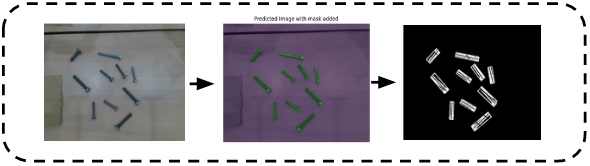
\includegraphics[width=\columnwidth]{results.png}
%\epsfxsize=3.25in\epsfbox{figure1.epsi}
\caption{RGB image(left), segmented image(middle), bounding box with center line on binary image(right) of target objects.}
\label{results_1}
\end{figure}
\subsection{Localization of Bolts in Robot's Configuration}
Building upon the initial localization of bolts within the camera frame, a crucial next step involves transforming this information to the robot's coordinate system. This transformation is essential for enabling the robot arm to accurately grasp and sort the bolts based on their estimated size and orientation. From the information available in $F_{i}$, the position of each bolt is transformed to the robot's base. As shown in Fig. \ref{experimental_Setup}, the camera and robot are at predefined positions. Considering the camera's pose(orientation and translation) with respect to the robot's base, the transformation matrix is denoted as $T_{C}^{B}$ in Eq. \ref{Camera_transformation}.
\begin{figure}[h!]
\centering
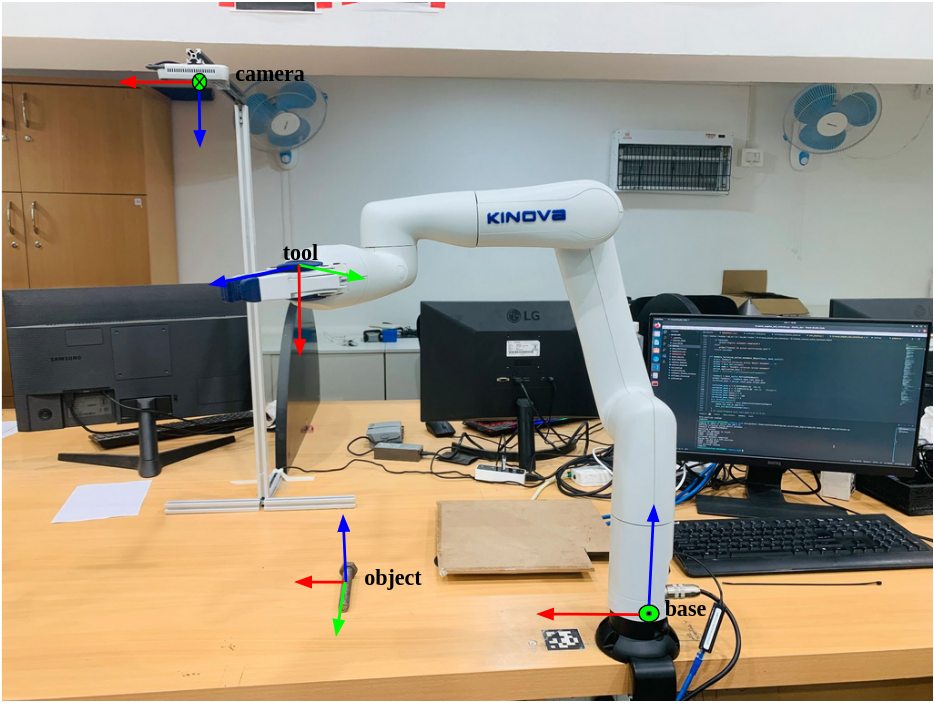
\includegraphics[width=0.75\columnwidth]{setup.png}
%\epsfxsize=3.25in\epsfbox{figure1.epsi}
\caption{Visual servoing experiment setup.}
\label{experimental_Setup}
\end{figure}
\begin{equation}
\text{$T^{B}_{C}$} =
\begin{bmatrix}
1 & 0 & 0 & 0.48\\
0 & -1 & 0 & -0.27\\
0 & 0 & -1 & 0.75\\
0 & 0 & 0 & 1\\
\end{bmatrix}
\label{Camera_transformation}
\end{equation}
$P_{O}^{C}$ is the position of the object with respect to the camera.
\begin{equation}
P_{O}^{C} = \begin{bmatrix} X & Y & Z & 1 \end{bmatrix}^T
\label{position_object_camera}
\end{equation}
Position of object with respect robot base can be defined by 
\begin{equation}
    P_{O}^{B} = T_{C}^{B} \cdot P^{C}_{O}
    \label{final_transformation}
\end{equation}
where $P_{O}^{B}$ is 
\begin{equation}
P_{O}^{B} = \begin{bmatrix} X' & Y' & Z' & 1 \end{bmatrix}^T
\label{position_object_base}
\end{equation}
We can extend for 'n' number of bolts as shown in Eq. \ref{position_object_base}.
\begin{equation}
\begin{bmatrix}
{X'_{1}}^{B} \ldots & {X'_{n}}^{B}\\
{Y'_{1}}^{B} \ldots & {Y'_{n}}^{B}\\
{Z'_{1}}^{B} \ldots & {Z'_{n}}^{B}\\
1 \ldots & 1\\
\end{bmatrix}
\text{=}
\begin{bmatrix}
1 & 0 & 0 & 0.48\\
0 & -1 & 0 & -0.27\\
0 & 0 & -1 & 0.75\\
0 & 0 & 0 & 1\\
\end{bmatrix} \cdot
\begin{bmatrix}
X_{1}^{B} \ldots & X_{n}^{B}\\
Y_{1}^{B} \ldots & Y_{n}^{B}\\
Z_{1}^{B} \ldots & Z_{n}^{B}\\
1 \ldots & 1\\
\end{bmatrix}
\label{position_object_base}
\end{equation}

\begin{figure}
\centering
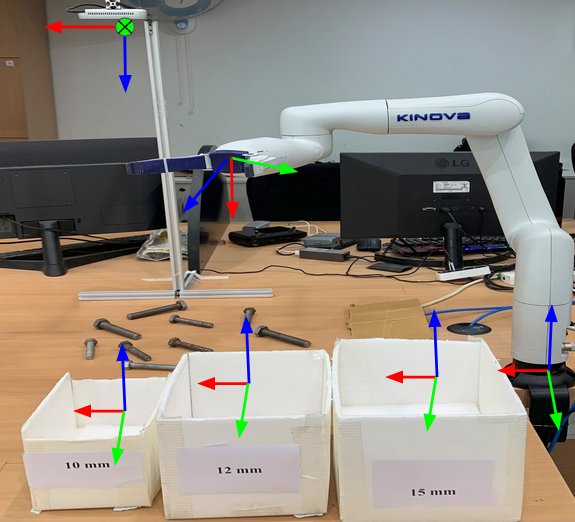
\includegraphics[width=0.75\columnwidth]{fina_experiment_setup.png}
%\epsfxsize=3.25in\epsfbox{figure1.epsi}
\caption{Experimental setup to test our methodology for sorting bolts.}
\label{final_setup}
\end{figure}
\section{Experimental Setup \& Results}
\begin{table}[htbp]
\caption{Comparison of Actual and Predicted Values from Methodology}
\begin{center}
\renewcommand{\arraystretch}{1.2} % Adjust row height
\rowcolors{2}{gray!25}{white} % Alternate row colors
\begin{tabular}{|c|c|c|c|c|}
    \hline
    \textbf{S.No} & \textbf{Type} & \textbf{Actual (mm)} & \textbf{Predicted (mm)} & \textbf{Error (mm)}\\ 
    \hline
    1 & M15 & 15 & 14.727 & 0.273\\
      &    &    & 14.333 & 0.667\\
      &    &    & 16.424 & 1.424\\
      &    &    & 13.345 & 1.655\\
    \hline
    \hline
    2 & M12 & 12 & 11.743 & 0.273\\
      &    &    & 12.290 & 0.290\\
      &    &    & 12.033 & 0.033\\
      &    &    & 10.833 & 1.167\\
    \hline
    \hline
    3 & M10 & 10 & 10.179 & 0.179\\
      &    &    & 10.210 & 0.210\\
      &    &    & 9.920 & 0.080\\
      &    &    & 10.280 & 0.280\\
    \hline
    \hline
    4 & M8  & 8  & 8.271 & 0.271\\
      &    &    & 7.173 & 0.827\\
      &    &    & 8.767 & 0.767\\
      &    &    & 7.893 & 0.107\\
    \hline
  \end{tabular}
\label{Table2}
\end{center}
\end{table}

\begin{figure}[h!]
\centering
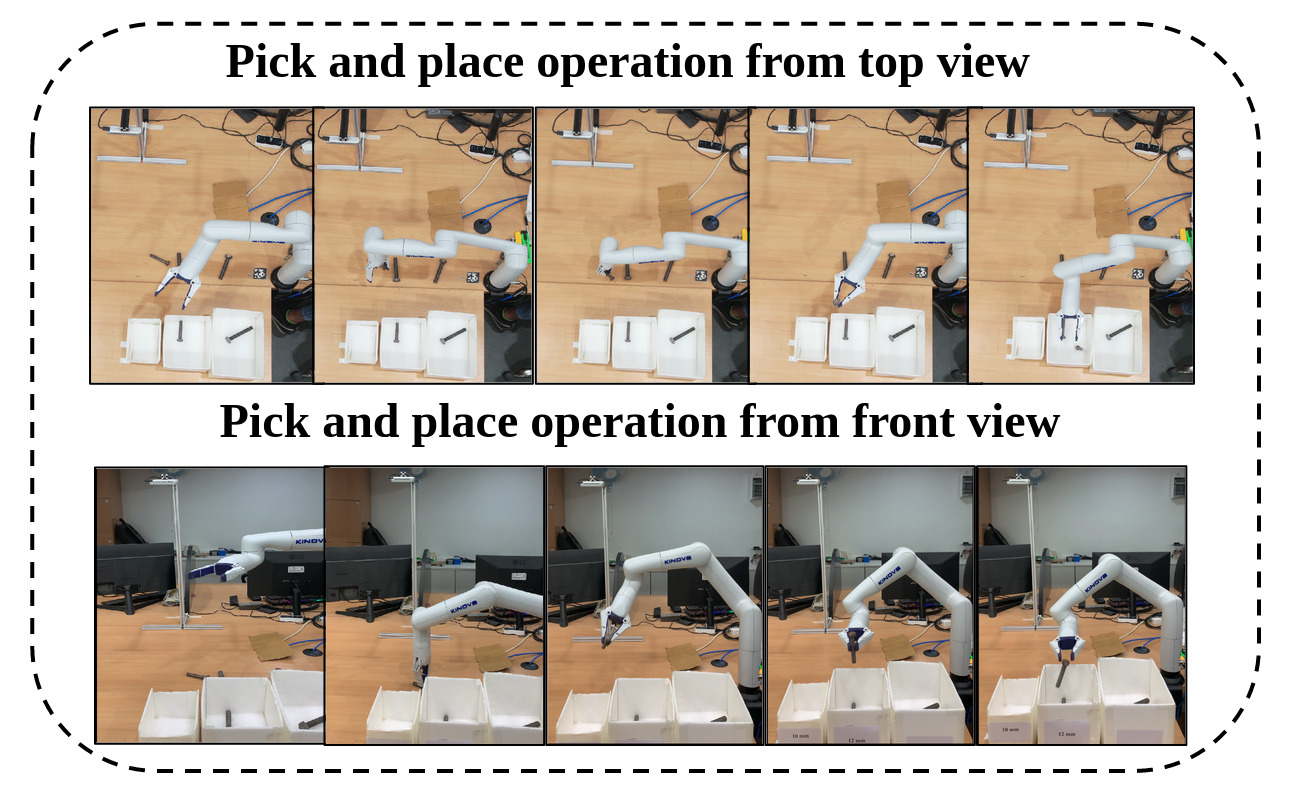
\includegraphics[width=\columnwidth]{end_results.jpg}
%\epsfxsize=3.25in\epsfbox{figure1.epsi}
\caption{Picking and placing bolt in their respective bins(Sorting).}
\label{results}
\end{figure}
The methodology developed for our custom data is tested using an experimental setup as shown in Fig. \ref{final_setup}. We established a TCP/IP Ethernet connection using a server-client architecture to facilitate communication between the CPU and the robot arm. This connection allows the CPU to send control commands and receive status updates from the robot arm. The CPU used for the experiment and model training is an Intel NUC9i9QNX Kit with 32 GB of RAM. By leveraging functionalities within the Kinova API package, we achieved the desired task of automated bolt sorting. We placed bins at predefined locations with respect to the robot base to accommodate bolts. All bolts were placed in unorganized positions within the field of view of our global camera. The robot was able to reach the object by aligning its end effector according to the bolt's pose and completed the sorting operation using criteria set heuristically in Eq. \ref{criteria}, placing bolts in their respective bins as shown in Fig. \ref{results}. Furthermore, we introduced new-sized bolts that were not used for training our model. Our methodology was able to estimate their size and complete the sorting operation successfully.
\begin{equation}
\text{bolt}=
    \begin{cases}
        \text{M15} & \text{if } 13.5 \leq \text{d} < 16.5 \\
        \text{M12} & \text{if } 10.5 \leq \text{d} < 12.5 \\
        \text{M10} & \text{if } 9.5 \leq \text{d} < 10.3 \\
        \text{M8} & \text{if }  7.0 \leq \text{d} < 8.5 \\
    \end{cases}
    \label{criteria}
\end{equation}

\section{CONCLUSIONS}
In this paper, we systematically evaluated state-of-the-art deep learning models for semantic segmentation on our custom dataset of bolts. DeepLabV3+ performed best for optimized masking of bolts. By amalgamating classical vision techniques with the segmentation model, we were able to estimate bolt sizes precisely with an error range of (-1.424, 1.655) mm. We experimentally validated the localization and size estimation by performing a sorting task using the Kinova Gen3 Lite arm. Through a series of experiments, we were able to perform sorting without any misclassifications (Video link). This work demonstrates a promising approach to enhancing automation in industrial settings and warehouse management. By integrating deep learning and classical vision techniques, we provide a solution that could potentially improve the accuracy and efficiency of sorting tasks, contributing to more streamlined operations. In our present experiment, we assumed the object to be static and used an in-built gripper. In the future, we aim to handle objects in overlapping or occluded configurations, as well as moving objects, and reduce the sorting time with a customized gripper. Additionally, we plan to extend our work to include nuts, which will be useful for the assembly of nuts and bolts using a dual-arm manipulator.
\section*{ACKNOWLEDGMENT}
In this work, Smrithi S., an intern from the Centre for AI and Robotics at IIT Mandi, provided her valuable support by exploring methods to incorporate depth camera data for improved size estimation.
\bibliographystyle{ieeetr}
\bibliography{ref}
\end{document}
